\documentclass[border=12pt]{standalone}
\usepackage{tikz}
\usetikzlibrary{shapes.geometric, arrows.meta, positioning, calc, fit, backgrounds}
\usepackage{fontspec}
\setmainfont{DejaVu Sans}

\begin{document}
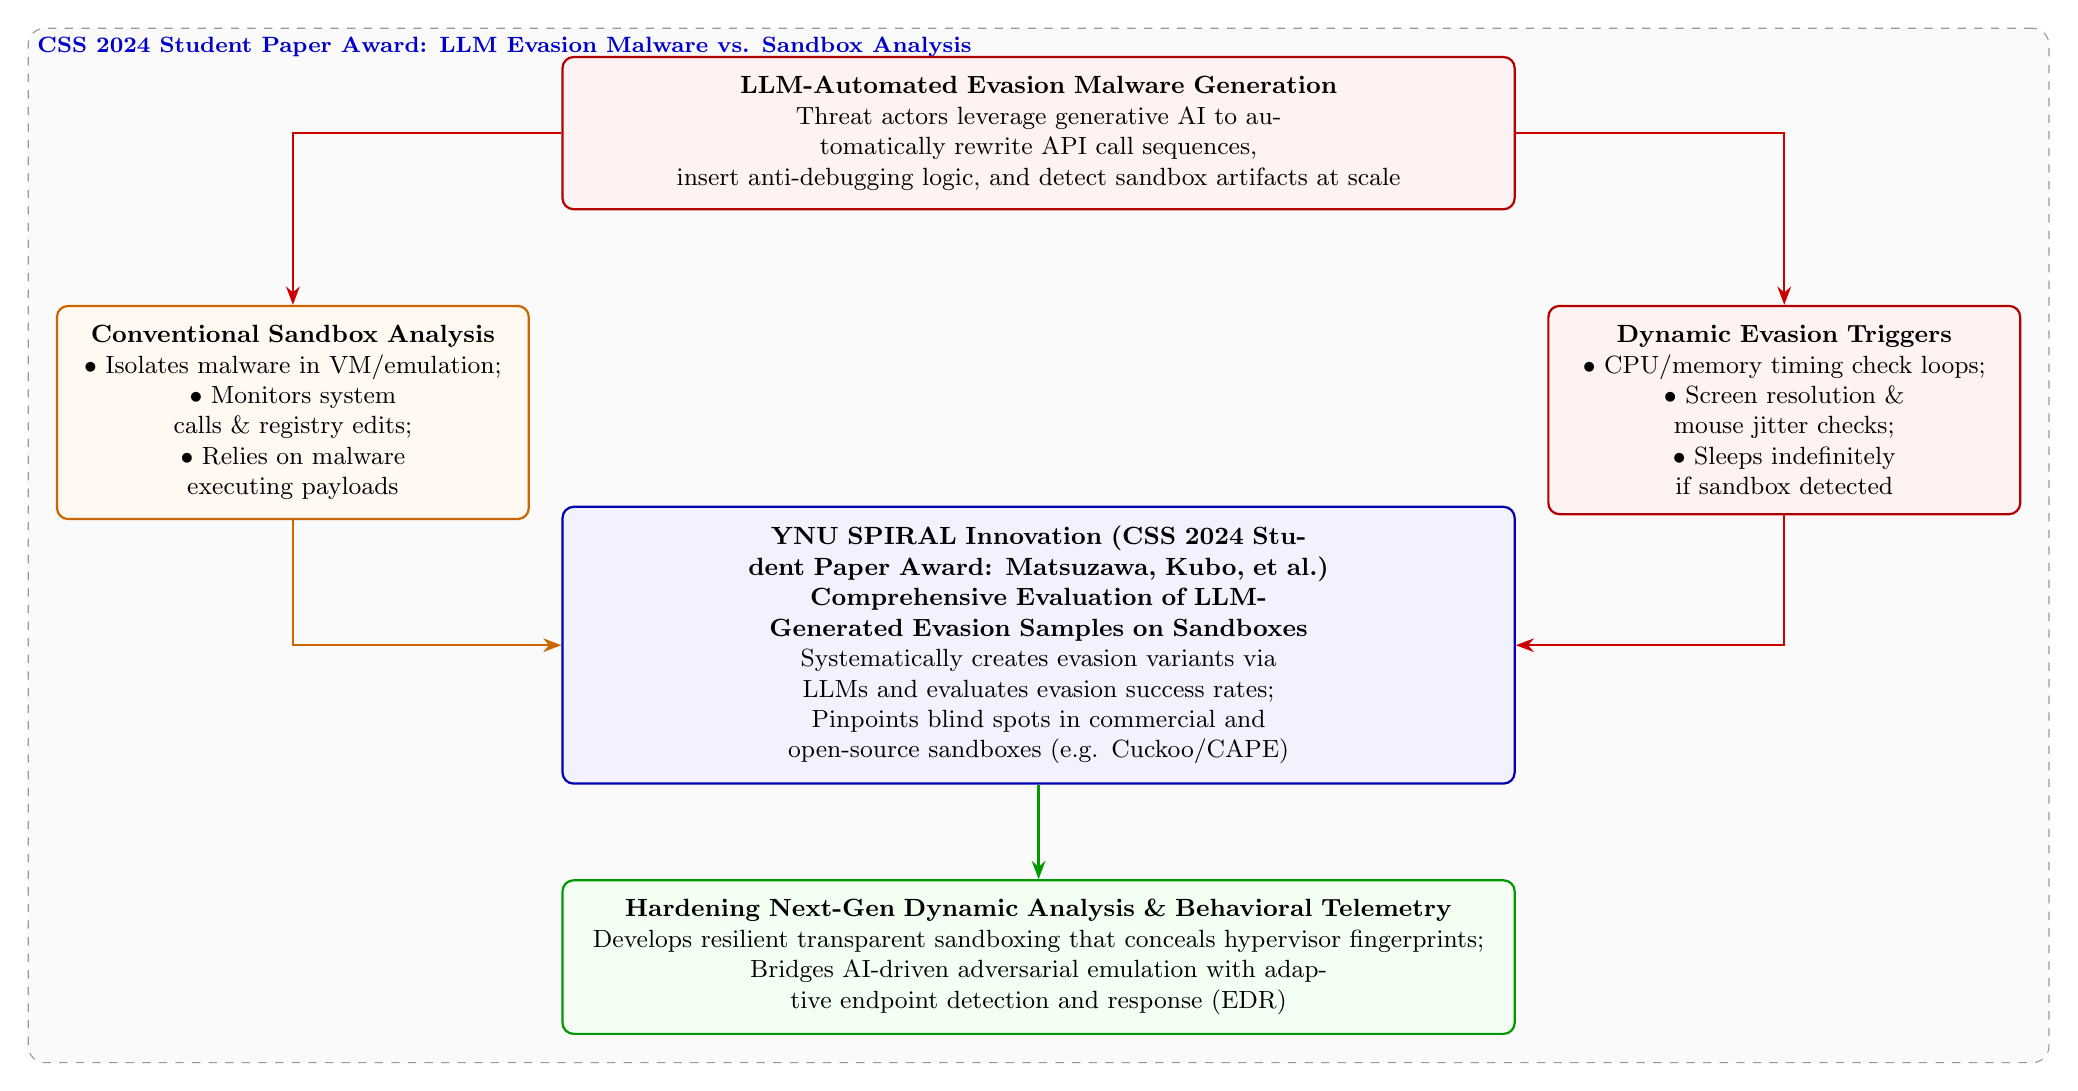
\begin{tikzpicture}[
    font=\small,
    >=Stealth,
    node distance=1.2cm,
    block/.style={rectangle, draw=blue!70!black, fill=blue!5, rounded corners=4pt, thick, align=center, inner sep=7pt},
    alertblock/.style={rectangle, draw=red!70!black, fill=red!5, rounded corners=4pt, thick, align=center, inner sep=7pt},
    greenblock/.style={rectangle, draw=green!60!black, fill=green!5, rounded corners=4pt, thick, align=center, inner sep=7pt},
    amberblock/.style={rectangle, draw=orange!80!black, fill=orange!5, rounded corners=4pt, thick, align=center, inner sep=7pt},
    groupbox/.style={draw=black!40, dashed, rounded corners=6pt, fill=black!2, inner sep=10pt}
]

    % Top: The Rise of LLM-Driven Polymorphic Evasion
    \node[alertblock, text width=11.6cm] (llm) {\textbf{LLM-Automated Evasion Malware Generation}\\Threat actors leverage generative AI to automatically rewrite API call sequences,\\insert anti-debugging logic, and detect sandbox artifacts at scale};

    % Left: Traditional Sandbox Dynamics
    \node[amberblock, below left=1.2cm and 0.4cm of llm, text width=5.5cm] (sandbox) {\textbf{Conventional Sandbox Analysis}\\$\bullet$ Isolates malware in VM/emulation;\\$\bullet$ Monitors system calls \& registry edits;\\$\bullet$ Relies on malware executing payloads};

    % Right: LLM Evasion Techniques
    \node[alertblock, below right=1.2cm and 0.4cm of llm, text width=5.5cm] (techniques) {\textbf{Dynamic Evasion Triggers}\\$\bullet$ CPU/memory timing check loops;\\$\bullet$ Screen resolution \& mouse jitter checks;\\$\bullet$ Sleeps indefinitely if sandbox detected};

    \draw[->, thick, red!80!black] (llm) -| (sandbox);
    \draw[->, thick, red!80!black] (llm) -| (techniques);

    % Middle: YNU Breakthrough (CSS 2024 Student Paper Award)
    \node[block, below=1.2cm of $(sandbox)!0.5!(techniques)$, text width=11.6cm] (breakthrough) {\textbf{YNU SPIRAL Innovation (CSS 2024 Student Paper Award: Matsuzawa, Kubo, et al.)}\\\textbf{Comprehensive Evaluation of LLM-Generated Evasion Samples on Sandboxes}\\Systematically creates evasion variants via LLMs and evaluates evasion success rates;\\Pinpoints blind spots in commercial and open-source sandboxes (e.g. Cuckoo/CAPE)};

    \draw[->, thick, orange!80!black] (sandbox) |- (breakthrough);
    \draw[->, thick, red!80!black] (techniques) |- (breakthrough);

    % Bottom: Future Defense Impact
    \node[greenblock, below=1.2cm of breakthrough, text width=11.6cm] (impact) {\textbf{Hardening Next-Gen Dynamic Analysis \& Behavioral Telemetry}\\Develops resilient transparent sandboxing that conceals hypervisor fingerprints;\\Bridges AI-driven adversarial emulation with adaptive endpoint detection and response (EDR)};

    \draw[->, thick, green!60!black] (breakthrough) -- (impact);

    \begin{scope}[on background layer]
        \node[groupbox, fit=(llm) (sandbox) (techniques) (breakthrough) (impact), label={[anchor=north west, font=\footnotesize\bfseries, blue!80!black]north west:CSS 2024 Student Paper Award: LLM Evasion Malware vs. Sandbox Analysis}] {};
    \end{scope}

\end{tikzpicture}
\end{document}
